%%Aquí se se describe a parte experimental de la tesis

De los métodos mencionados en el capítulo \ref{EdArt} se procedió a realizar una verificación con la finalidad de obtener resultados parciales similares a los obtenidos por los autores, se llevó a cabo la implementación de los métodos más importantes, entre ellos la forma de medir el campo de profundidad a partir de modificar la distancia focal.

Los experimentos se llevó a cabo en un conjunto de imágenes integrado por 27 elementos, los cuales a traves de cada uno de ellos el campo de profundidad presenta una variación, dando lugar a que ciertas zonas presenten niveles de borrosidad distintos, o en su caso contrario, niveles de nitidez distinto. En los métodos que se procede, se muestran métricas para poder evaluar la cantidad de nitidez en cada una de las imágenes.

\begin{figure}
\centering
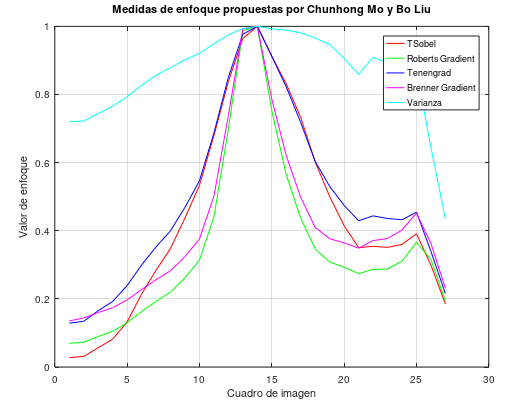
\includegraphics[width=\textwidth]{GraficosExperimentacion/sobelSinRuido.PNG}
\caption{Gráficas de los valores de evaluación normalizados en \citet{Mo2012} aplicados a Zebra sin ruido. }
\label{SalidaTSobelSinRuido}
\end{figure}

 Primeramente se recurre al método planteado por \citet{Mo2012} donde toma el conjunto de imágenes como datos de entrada y  un valor de evaluación como datos de salida, el autor realiza la comparación de éste método con respecto a otros, lo esperado tras realizar esta experimentación es obtener unos resultados similares al autor, donde el algoritmo propuesto llamado Sobel mejorado da los mejores resultados. 
\\
\\
Se realizaron pruebas con el conjunto de imágenes Zebra con y sin ruido. El ruido se generó de de manera artificial y se le sumó a cada una de las imágenes previo a realizar los cálculos sobre ellas, los resultados se muestran en la figura \ref{SalidaTSobelSinRuido} de los valores normalizados por cada uno de los métodos mencionados en \citet{Mo2012}, donde el algoritmo Sobel mejorado se pinta de color rojo.

\begin{figure}
\centering
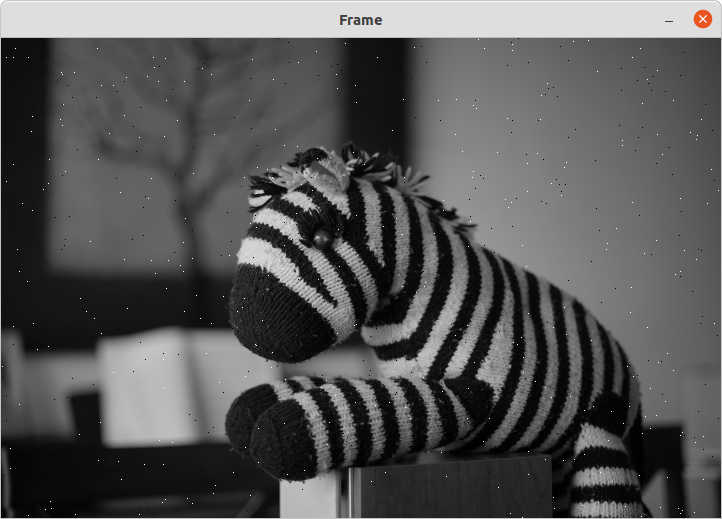
\includegraphics[width=\textwidth]{GraficosExperimentacion/CebraConRuidoFOCUS.png}
\caption{Resultado de imagen tras aplicar ruido de sal y pimienta.}
\label{cebraRuido}
\end{figure}

Posteriormente a ello se realizó el mismo experimento pero con la adición del ruido, en este caso se trató de un ruido sal y pimienta (vease en la figura \ref{cebraRuido}) y la salida del programa se muestra en forma de gráfica, mostrada en la figura \ref{SalidaTSobelConRuido}. Como se puede apreciar, existe un comportamiento similar al ilustrado en la figura \ref{FocusingWithNoise_mo2012} en donde todas las curvas se desplazan hacia arriba, de tal forma que el rango de valores de enfoque gira entre los 0.85 y 1 a diferencia de lo ilustrado en la gráfica \ref{SalidaTSobelSinRuido} cuyos valores de enfoque van entre 0.01 y 1.

 
\begin{figure}
\centering
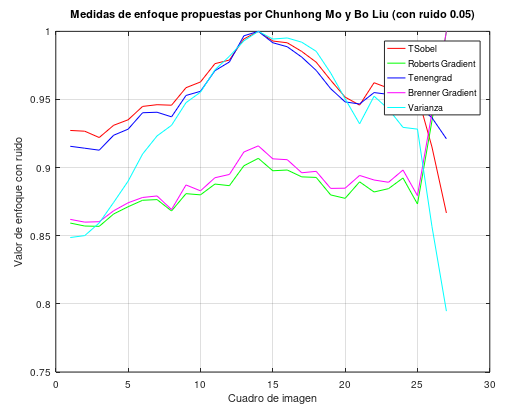
\includegraphics[width=\textwidth]{GraficosExperimentacion/sobelRuido.PNG}
\caption{Gráficas de los valores de evaluación normalizados en \citet{Mo2012} aplicados a Zebra con ruido. }
\label{SalidaTSobelConRuido}
\end{figure}


En \citet{Subbarao1993} se llevó a cabo una implementación de los métodos propuestos, donde la finalidad de estos es medir la cantidad de enfoque en una imagen, algunas de las métricas propuestas trabajan en el dominio de las frecuencias, por lo que el autor compara los resultados obtenidos tras medir un mismo conjunto de imágenes bajo su dominio original y en su dominio de frecuencias.






















